% !Mode:: "TeX:UTF-8"
%\documentclass[twocolumn]{sig-alternate}
%\documentclass[letterpaper, twocolumn]{sig-alternate-10pt}
%\documentclass[twocolumn,10pt]{infocom}
%\documentclass[twocolumn,10pt]{IEEEtran_v15}
%\documentclass[twocolumn,10pt]{IEEEtran}
%\documentclass[twocolumn,10pt]{article}
%\usepackage[sort,nocompress,space]{cite}
\documentclass{sig-alternate-10pt}
%\documentclass[letterpaper,twocolumn,10pt]{article}
\usepackage{epsfig,endnotes}
%\usepackage[letterpaper]{geometry}

\usepackage[export]{adjustbox}

%\usepackage{ifpdf}
%\ifpdf
%\setlength{\pdfpagewidth}{8.5in}
%\setlength{\pdfpageheight}{11in}
%\else
%\fi

%%%%%%%%%%%%%%%%%%%%%%
% Set Compact Mode   %
%%%%%%%%%%%%%%%%%%%%%%

%\newcommand{\subparagraph}{}


%\usepackage[compact]{titlesec}
%\titlespacing{\section}{0pt}{*0}{*0}
%\titlespacing{\subsection}{0pt}{*0}{*0}
%\titlespacing{\subsubsection}{0pt}{*0}{*0}
%\setlength{\parskip}{0pt}
%\setlength{\parsep}{0pt}
%\setlength{\headsep}{0pt}
%\setlength{\topskip}{0pt}
%\setlength{\topmargin}{0pt}
%\setlength{\topsep}{0pt}
%\setlength{\partopsep}{0pt}
%\setlength{\itemsep}{0pt}

%%%%%%%%%%%%%%%%%%%%%%
%
%%%%%%%%%%%%%%%%%%%%%%


\usepackage{url}
\usepackage[sort,space]{cite}
\usepackage{lineno}
\renewcommand\linenumberfont{\normalfont\bfseries\small}
\usepackage{pifont}
\usepackage{epsfig,epsf,url,amssymb}
\usepackage{tabularx}
%\usepackage{algorithm2e}
\usepackage[ruled,vlined]{algorithm2e}
\usepackage{algpseudocode}
\usepackage{amsmath}
\usepackage{mathtools}
\newtheorem{mydef}{Definition}
\usepackage{rotating}
\usepackage{wrapfig}
\usepackage{times}
\long\def\comment#1{}
\usepackage{multirow}
\usepackage{lscape}
\usepackage{stmaryrd}
\usepackage{wrapfig}
\usepackage{hhline}
\usepackage{textcomp,booktabs}
\usepackage[usenames,dvipsnames]{color}
\usepackage{colortbl}
\usepackage{multirow}
\usepackage{rotating}
\usepackage{epstopdf}
\usepackage[tight,footnotesize]{subfigure}

%\usepackage{hyperref}
\usepackage{url}
\definecolor{mygray}{gray}{.9}
\definecolor{mypink}{gray}{.9}
\definecolor{mycyan}{cmyk}{.3,0,0,0}

\usepackage{graphicx}
%\usepackage{subfigure}
\usepackage{subfig}
\usepackage[font=bf]{caption}

\newcommand{\bbR}{\mathbb{R}}
\newcommand{\calN}{\mathcal{N}}
\newcommand{\calR}{\mathcal{R}}
\newcommand{\calV}{\mathcal{V}}
\newcommand{\eg}{{\it e.g.}}
\newcommand{\etal}{{\it et al.~}}
\newcommand{\etc}{{\it etc.}}
\newcommand{\ie}{{\it i.e.}}
\newcommand{\tablecapspace}{{\vspace{-0.1in}}}
\newcommand{\tablespace}{{\vspace{-0.05in}}}
\newcommand{\picspace}{{\vspace{-0.1in}}}
\renewcommand{\baselinestretch}{1}
\renewcommand{\arraystretch}{1.05}      % make the space between tabular lines larger
\newcommand{\capspace}{}           % control space between figure/table and caption
\newcommand\fixme[1]{{\color{red} #1}}
\newcommand{\secspace[1]}{\vspace{-0.06in}}


\newcommand{\para}[1]{{\vspace{3pt} \bf \noindent #1 \hspace{6pt}}}

\def\TODO#1{\textcolor{red}{}}
%\setlength{\textheight}{9.3in}
%\setlength{\columnsep}{1.4pc}
%\setlength{\textwidth}{7.1in}

\newcommand{\sys}{{\textrm{XPath}}\xspace}

\newcommand{\paragraphb}[1]{\vspace{0.05in}\noindent{\bf #1}}

\newcommand{\paraspace}{\vspace{0.05in}}
\newcommand{\parab}[1]{\paraspace\noindent{\bf #1} }
\newcommand{\parae}[1]{\paraspace\noindent{\em #1} }
\newcommand{\parabe}[1]{\paraspace\noindent{\bf \em #1} }
%\newcommand{\kai}[1]{{\color{blue}[Kai: #1]}}
\newcommand{\todo}{\textcolor{red}}

\def\naive{na\"\i ve}

\newcommand{\tabincell}[2]{\begin{tabular}{@{}#1@{}}#2\end{tabular}}

\newcommand{\subcaption}[1]{\centerline{#1}\vspace{0.1in}}
\long\def\comment#1{}
\newtheorem{theorem}{Theorem}
\newtheorem{lemma}[theorem]{Lemma}
\newtheorem{proposition}[theorem]{Proposition}
\newtheorem{corollary}[theorem]{Corollary}
%\newtheorem{problem}[theorem]{Problem}

\newenvironment{definition}[1][Definition]{\begin{trivlist}
\item[\hskip \labelsep {\bfseries #1}]}{\end{trivlist}}
\newenvironment{problem}[1][]{\begin{trivlist}
\item[\hskip \labelsep {\bfseries}]}{\end{trivlist}}
\newenvironment{remark}[1][Remark]{\begin{trivlist}
\item[\hskip \labelsep {\bfseries #1}]}{\end{trivlist}}

\newenvironment{icompact}{
  \begin{list}{$\bullet$}{
    \parsep 1pt plus 1pt
    \partopsep 1pt plus 1pt
    \topsep 1pt plus 2pt minus 1pt
    \itemsep 1.5pt plus 1pt
    \parskip 0pt plus 2pt
    \leftmargin 0.15in}
       }
  {\normalsize\end{list}}

\newenvironment{ecompact}{
  \begin{list}{$\bullet$}{
    \parsep 1pt plus 1pt
    \partopsep 1pt plus 1pt
    \topsep 1pt plus 2pt minus 1pt
    \itemsep 1.5pt plus 1pt
    \parskip 0pt plus 2pt
    \leftmargin 0.15in}
       }
  {\normalsize\end{list}}

%\hyphenpenalty=5000 %\tolerance=1000

%\hyphenation{Mega-Switch para-digm}


%%%%%%%% to calculate the time %%%%%%%%%%%%%%%%%%%%%%%%%%%%
\newcount\hour \newcount\minute
\hour=\time  \divide \hour by 60
\minute=\time
\loop \ifnum \minute > 59 \advance \minute by -60 \repeat
\def\drafttime{\ifnum \hour<13 \number\hour:%
                      \ifnum \minute<10 0\fi
                      \number\minute
                      \ifnum \hour<12 \ AM\else \ PM\fi
         \else \advance \hour by -12 \number\hour:%
                      \ifnum \minute<10 0\fi
                      \number\minute \ PM\fi}
\def\timestamp{\today \ \drafttime}

\begin{document}
%\conferenceinfo{SIGCOMM,} {XXXXXX, XXXXX, XXXXX, XXXXX.} %
%\CopyrightYear{2009} \crdata{1-59593-308-5/06/0009}

\title{Deadlocks in Datacenter Networks: Why Do They Form, and How to Avoid Them}
\author{Paper \#67}
\maketitle

%\vspace{-0.2in}
\abstract{
Driven by the need for ultra-low latency, high throughput and low CPU overhead,
Remote Direct Memory Access (RDMA) is being deployed by many cloud providers.
To deploy RDMA in Ethernet networks, Priority Flow Control (PFC) must be
used. PFC, however, makes Ethernet networks prone to deadlocks. Prior work on
deadlock avoidance has focused on {\em necessary} condition for deadlock
formation, which leads to rather onerous and expensive solutions for deadlock
avoidance. In this paper, we investigate {\em sufficient} conditions for
deadlock formation, conjecturing that avoiding {\em sufficient} conditions might
be less onerous.
}

%\vspace{-0.1in}
\section{Introduction}\label{sec:intro}

\para{Datacenter appliations demand high performance from the network. RDMA provides such performance.
We deploy RDMA over Converged Ethernet (RoCE).} \\ 

\para{RoCE relies on PFC. PFC can cause deadlocks.} \\

\para{Prior work} proposes theoritical solutions. But none of them is practical for current datacenter deployment.
There are two main issues, 1) most of the solutions require significant changes on routing, enforcing or accurately predicting
the path of each packet. This is conflicted with the nature of Ethernet and IP networks and hard to achieve in practice.
We have evidences from production datacenters that a certain portion of packets are routed unexpectedly, though not dropped.
2) The number of lossless priority available is very limited. There are only several traffic classes in total,
and each lossless class requires siginifant reserved buffer to make PFC work. 

\para{(Our solution)} In this paper, we work on a practical solution that can immediately implemented by 
commodity switches. We do not enforce the path of each packet or make any changes on the routing algorithm. 
This is important for network operators. We also minimize the hardware resources usage, like number of priority
classes, reserved buffer and number of ACL rules.

\para{(Limit the scope)} We do not discuss centralized SDN solutions. BTW, the centralized solution is not trivial, refer
to our hotnets paper. We assume our networks rely on PFC. These solutions would require significant changes 
in the network, and may affect performance.

\para{Specifically,} we seek to design an algorithm that takes the topology and routes that must be lossless as the 
input, and outputs the buffer configuration and ACL rules that guarantee no deadlock. To begin with, we focus on 
common structured datacenter topology, including Fat-tree and BCube. The key idea is to tag the packets along 
the path, and assign each packet to different lossless queues. Properly configured, we can eliminate any
possibilities of deadlock with a small number of lossless queues.

\para{We further extend our algorithms in two directions.} First, we consider generic, unstructured topology. 
We abstract the ideas in designing algorithms for strucutred topology, and develop an algorithm that works for
any graph, using TTL as a generic tag. We show that it works well for random topology like Jellyfish.
Second, in cases where the limit number of lossless queues cannot guarantee deadlock-free, we provide suggestions for 
network operator that which part of routing paths may be turned into lossy so that the whole network can be deadlock-free.

\para{We implement our algorithm and verify it using testbed and NS-3 simulations.} \\

\para{Our contributions.} 1) we analyze the practical challenges in making RoCE deadlock-free, including 
the challenges in enforcing/predicting routing and the limit of lossless queues. 2) we develop practical solutions
that eliminate deadlock for Fat-Tree and BCbue. 3) we extend our algorithm for generic graphs and scenarios
where the number of lossless queues is insufficient.



\section{Deadlock in Lossless Network}

In this section, we explain the background of deadlock in lossless network, and 
why we must study the necessary and sufficient condition of it.

\para{Lossless Ethernet relies on PFC.} 
Modern data center networks require efficient network stacks in order to support 
40Gbps or even higher bandwidth. RDMA over Ethernet, or RoCE, is the most popular
solution and has been deployed in both Google and Microsoft data centers~\cite{dcqcn, timely}.
The key property of such network is that it runs on lossless Ethernet, meaning
that no packet is dropped due to congestion. This is realized by PFC 
(Priority-based Flow Control).

PFC introduces PAUSE mechanism, with which the switch can pause an incoming link
when its ingress buffer occupancy reaches a preset threshold. Properly tuned, the 
buffer will never overflow, and no packet will be dropped due to full buffer.
As shown below, deadlock may occur in such lossless networks.


\para{Deadlock definition.}
We define deadlock as a permanent state in which a subset of links are all paused
by PFC, and none of the packets in the involved buffers can ever move even there is 
no more packet being sent into these links.

\para{PFC may lead to deadlock, if PFC-paused links form a circle.}
In a PFC-enabled network, if a subset of links congest and the buffer usage reach
the PFC threshold at the same time, the links are all paused. If these links happen
to form a complete circle, the network has a deadlock. No packet can moves because 
the links are paused, even if there is no more new traffic injected into this circle.

This essentially means {\em cyclic buffer dependency}. Any one link is waiting for its next
hop to RESUME the link, while this depends on the buffer status of the next hop. However,
the next hop buffer depend on the next next hop and wait for the RESUME
so that it can send out packets to lower the buffer usage. This goes on, and in the end, 
any stuck buffer depends on itself to move, thus forming a deadlock.

To avoid deadlock, previous work has considered {\em deadlock-free routing}.

\para{Achieving deadlock-free routing has high price, and may not even be viable.} 
In previous work, to achieve deadlock-free routing is to completely avoid cyclic buffer dependency.
It is proved that cyclic buffer dependency-free is necessary and sufficient to deadlock-free.
However, ensuring there is always no cyclic buffer dependency is challenging.

First, deadlock-free routing largely limits the choice of topology. For example, TCP-bolt 
has lengthy discussion on the design of deadlock-free routing and propose certain topology and routing. 
In today's datacenter network, a common configuration is to only use Clos-style topology, which does 
not have cyclic buffer dependency problem when the topology is complete. However, a number
of other topology setups are not cyclic buffer dependency-free.

Second, upon bugs or misconfiguration, deadlock-free routing configuration may become
vulnerable to deadlock. In fact, we have observed a deadlock case in our Clos network
deployment with PFC. (example here)


In this paper, we argue that we do not need to completely avoid cyclic buffer dependency.
Even if there is cyclic buffer dependency, deadlock may not occur (see Section~\ref{sec:xxx}).
This means that cyclic buffer dependency is a quite loose condition for deadlock.
We aim to explore a tighter condition, ideally a necessary and sufficient condition for deadlock.
Once we have better understanding, we may avoid deadlock with smaller price ({\em e.g.,} Section~\ref{sec:yyy}).



\section{Cyclic Buffer Dependency is insufficient for Deadlock}
\label{sec:analysis}

Although cyclic buffer dependency is a necessary condition for deadlock, it is not a
sufficient condition. In this section, we present our case studies in which cyclic 
buffer dependency is present, but deadlock occurrence still depends on other factors. We demonstrate 
that 1) a looping flow that generates cyclic buffer dependency does not always lead to deadlock. 
The length of loop, flow rates and packet Time-To-Live (TTL) affects whether 
the deadlock forms. 2) Multiple flows may cause cyclic buffer dependency,
but slightly different flow sets lead to different deadlock results. 3) Rate-limiting can
prevent deadlock from happening.

\subsection{Case 1: Flow Rate and TTL Determine Deadlock in a Routing Loop}

\begin{figure*}[t]
%\vspace{-0.1in}
\centering
\subfigure[Topology and flows.] {
    \includegraphics[width=0.37\textwidth] {figs/loop_case_topo_and_flow}
}
\subfigure[Buffer dependency graph.]{
    \includegraphics[width=0.28\textwidth] {figs/loop_case_ingress_buffer_dependency}
}
\subfigure[Stable state model.]{
    \includegraphics[width=0.28\textwidth] {figs/loop_analysis}
}
\caption{Single looping flow creates cyclic buffer dependency but may not create deadlock.}
\label{fig:loop}
\end{figure*}


A routing loop can create cyclic buffer dependency if a flow is trapped in the loop.
The simplest example is a two-hop loop between two switches, as shown in Figure~\ref{fig:loop}(a).
We then plot buffer dependency graph (Figure~\ref{fig:loop}(b)), $RX$ represents input 
queue (or port). Each directed line represents a buffer dependency from the source TX to the 
destination TX. For example, packets buffered in $RX1$ of switch A will be sent to either $RX1$ 
of B, and vice versa. So in Figure~\ref{fig:loop}(b), two directed lines are drawn between A and B.
Switch A's dependency on switch B means whether switch A can move
the packets in its receiving buffer {\em RX1} to egress depends on switch B's buffer {\em RX1}.\footnote{We 
focus on receiving buffer because PFC PAUSE triggers based on the occupancy of receiving buffer.}
The switches can send packets to the other side only 
when the other side's buffer utilization is under PFC PAUSE threshold. The deadlock happens when
both of the involved buffers reach the PFC threshold at the same time and PAUSE the links.  


However, this cyclic buffer dependency may not always turn into deadlock state. The flow
sending rate, the TTL (time-to-live) of packets and the length of the loop together 
determine whether there will be deadlock. In our testbed, we run a simple experiment on 
two switches that are connected by a 40Gbps link and configured with a routing loop. 
All packets have initial TTL of 16 and are injected into one of the switches. We find that, 
only if the packet injection rate exceeds 5Gbps, there can occur deadlock. 

In order to analyze deadlock occurrence in the cases of routing loop, we develop a mechanism called 
{\em boundary state analysis}. It yields accurate prediction of whether deadlock forms,
as shown below.

\para{Boundary state analysis.} 
On any of the switches in the loop, packets are injected by the previous hop and drained by the next hop. 
If the draining rate is smaller than the injecting rate, packets will continuously queue up in the
switch buffers. In a loop, once one switch buffers enough packets and triggers PFC, the PFC will soon
cascade through the whole loop and forms deadlock. 
We define {\em boundary state}, in which the injecting rate and draining rate are balanced on every
switch, and any larger injecting rate leads to deadlock because draining rate cannot catch up.

We build the boundary state model as illustrated in 
Figure~\ref{fig:loop}(c). The variables are described in Table~\ref{tab:stable_state}.


\begin{table}[h]
\centering
\caption{\small Stable state analysis variables}
\label{tab:stable_state}
{\small
\begin{tabular}{|c|c|}
 \hline
Variable &  Description \\
\hline
$r$ & Inject rate of new packets. \\
\hline
$B$ & Link bandwidth. \\
\hline
$r_d$ & Packets drain rate caused by TTL expiration. \\
\hline
$TTL$ & Initial Time-To-Live value. \\
\hline
$n$ & The length of the routing loop. \\
\hline
\end{tabular}
}
\end{table}

According to the boundary state definition, the injecting rate and draining rate
must be equal on the first switch:

\begin{equation}
\small
r + B - r_d = B
\label{eq:rate}
\end{equation}

In addition, we consider the sum of TTL values of all packets in the system. 
During the boundary state, it should remain stable. Therefore, the increase
rate and decrease rate of the sum of TTL should be the same:

\begin{equation}
\small
n * B = TTL * r
\label{eq:ttl}
\end{equation}

Combining Equation~\ref{eq:rate}, Equation~\ref{eq:ttl}, and the fact that
deadlock requires larger injecting rate than that in boundary state, we derive the 
{\em necessary and sufficient condition} of deadlock in a routing loop scenario:

\begin{equation}
\small
r > r_d = \frac{nB}{TTL}
\label{eq:condition}
\end{equation}

This matches what we observe in testbed experiment: with $B=40Gbps$, $n=2$ and
$TTL=16$, the flow injecting rate must be at least $5Gbps$ to cause deadlock. With larger bandwidth,
shorter loop length or smaller initial TTL values, the threshold of $r$ can be higher.
As long as the flow rate is smaller than the threshold, no deadlock will form.
As shown in Section~\ref{sec:mitigation}, we may utilize this property to avoid deadlock, 
even if routing loop occurs. 

\subsection{Case 2: Traffic Matrix Affects Deadlock}

Multiple flows may create a cyclic buffer dependency even if there is no routing loop.
Figure~\ref{fig:case1}(a) shows a simple example with four switches A, B, C and D. 
Flow 1 starts at a host (not shown) attached to A, passes through B and C, and ends at a 
host attached to D. Flow 2 starts at a host attached to C, passes through D and A, and 
ends at a host attached to B.
Similar to the previous case, we can draw the dependency lines between switches. As shown in 
Figure~\ref{fig:case1}(b), there is a cyclic buffer dependency among the four switches, i.e., 
dependencies from RX1 of A to RX1 of B, then to RX1 of C, then to RX1 of D, and finally back to RX1 of A.


In this example, the boundary state analysis does not yield meaningful
results. In fact, without any rate limiting on the flows, one can easily analyze that the 
stable throughput of each flow is $B/2$. However, it is not easy to tell whether deadlock 
will occur. For example, one may suspect that switch A's $RX1$ will generate PFC PAUSE, and 
these PAUSE frames may cascade from A to D, then to C, B and finally back to A, thus creating deadlock.
To understand such scenarios, we must analyze and simulate them at packet level.


\begin{figure*}[t]
%\vspace{-0.1in}
\centering

\subfigure[Topology and flows.] {
    \includegraphics[width=0.4\textwidth] {figs/case1_topo.pdf}
}
\subfigure[Buffer dependency graph.]{
    \includegraphics[width=0.24\textwidth] {figs/case1_buffer_dependency.pdf}
}
\subfigure[Pause events at four links.]{
    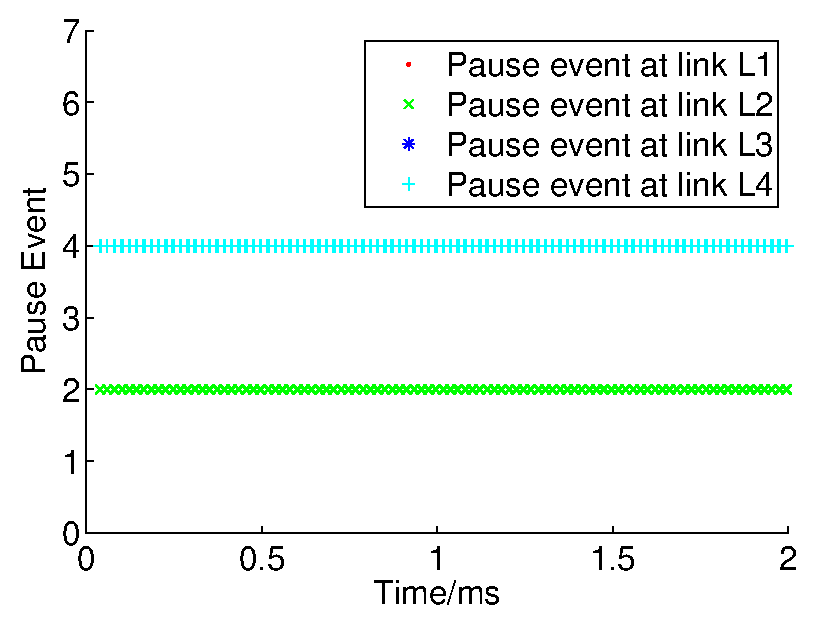
\includegraphics[width=0.3\textwidth] {figs/case1_pause.eps}
}

\subfigure[Buffer occupancy at switch A.] {
    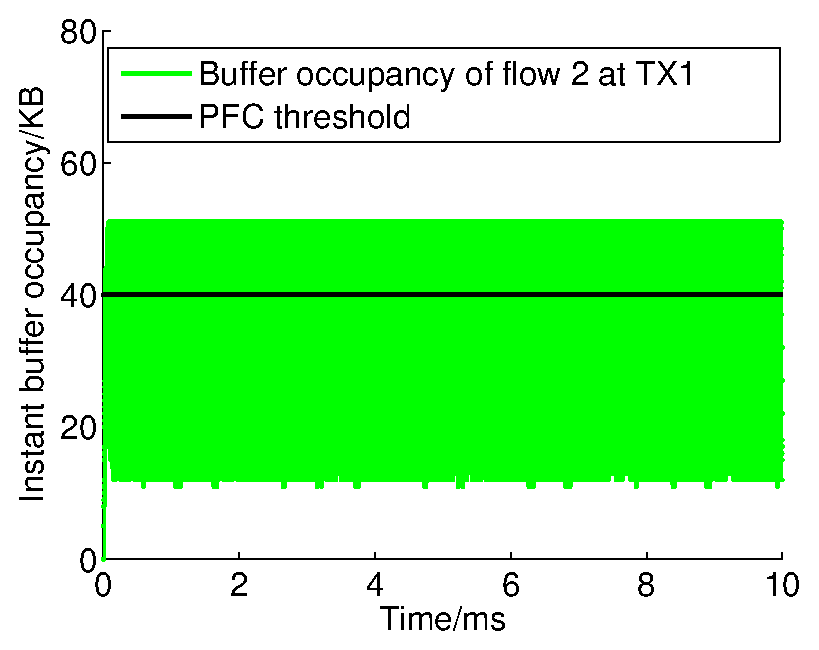
\includegraphics[width=0.23\textwidth] {figs/case1_buffer_occupancy_A.eps}
}
\subfigure[Buffer occupancy at switch B.] {
    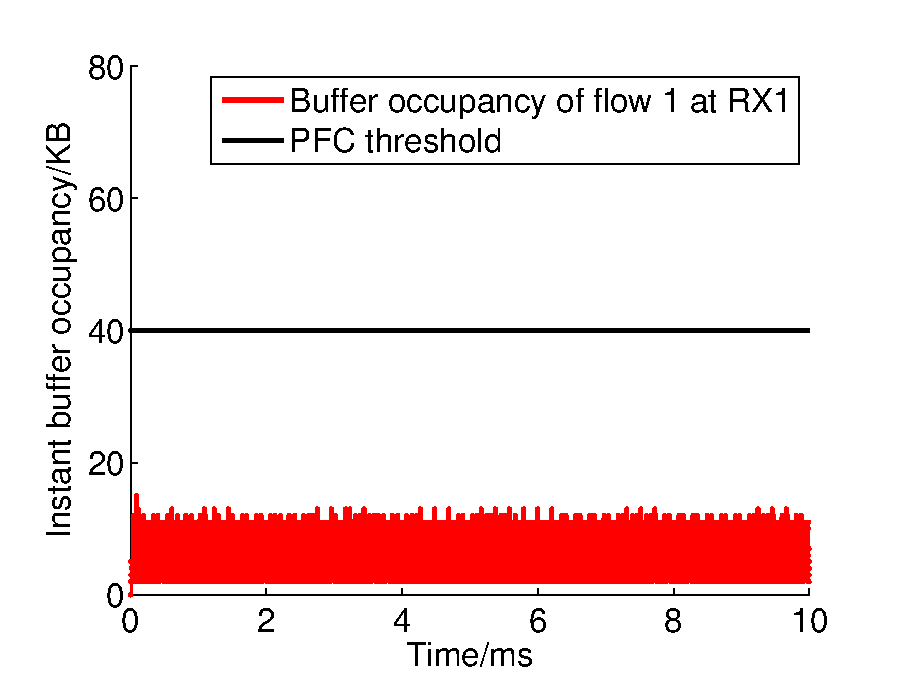
\includegraphics[width=0.23\textwidth] {figs/case1_buffer_occupancy_B.eps}
}
\subfigure[Buffer occupancy at switch C.] {
    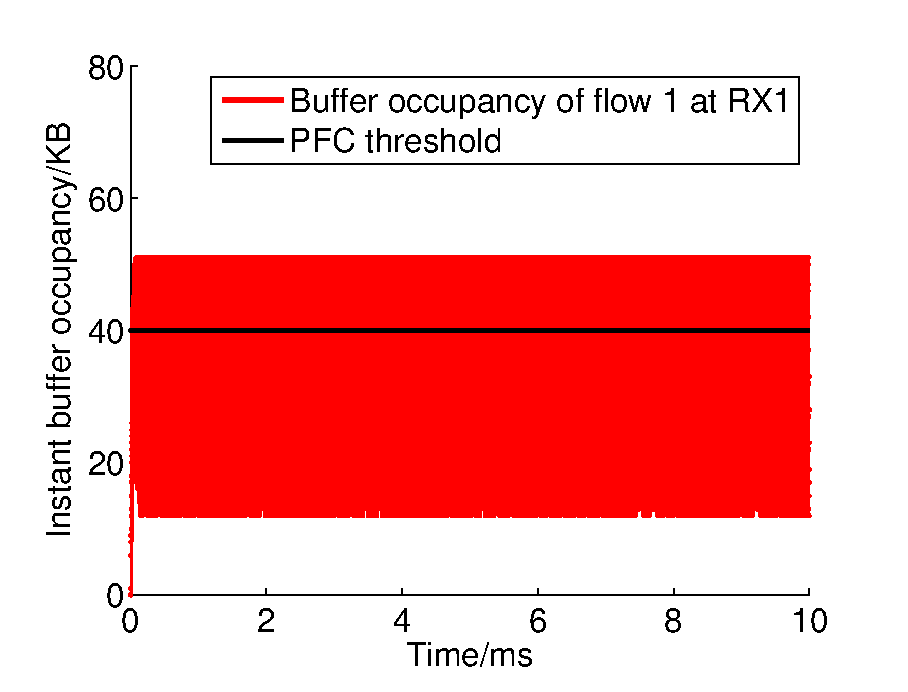
\includegraphics[width=0.23\textwidth] {figs/case1_buffer_occupancy_C.eps}
}
\subfigure[Buffer occupancy at switch D.] {
    \includegraphics[width=0.23\textwidth] {figs/case1_buffer_occupancy_D.eps}
}
\caption{There is no deadlock even though two flows create cyclic buffer dependency among four switches.}
\label{fig:case1}
\end{figure*}

 \textbf{Simulation setup}: To create a well controlled experimental environment, 
 we did our deadlock case study using packet-level NS-3 simulations. 
 
 In our modified NS-3 simulator, we implement PFC protocol ({\em i.e.,} IEEE 802.1 Qbb protocol). 
 Most modern commodity switches have a common shared buffer, while PFC works in a per ingress 
 queue fashion. For each ingress queue, the switch maintains a counter to 
 track its instant virtual queue length (i.e., bytes of buffered packets received by this 
 ingress queue). Once the queue length of an ingress queue exceeds the pre-configured PFC 
 threshold, a pause frame will be sent to the corresponding upstream device. The upstream 
 device then stop sending any packet to this ingress queue unless 1) the pause frame has 
 expired; 2) or it has received a resume frame from this ingress queue.


\begin{figure*}[t]
%\vspace{-0.1in}
\centering

\subfigure[Topology and flows.] {
    \includegraphics[width=0.37\textwidth] {figs/case2_topo}
}
\subfigure[Buffer dependency graph.]{
    \includegraphics[width=0.27\textwidth] {figs/case2_buffer_dependency}
}
\subfigure[Pause events at four links.]{
    \includegraphics[width=0.3\textwidth] {figs/case2_pause.eps}
}
\caption{Slightly different traffic matrix leads to deadlock, even though
the flow-level stable state analysis shows the rates of flow 1 and flow 2 should not affected.
On L3, flow-level analysis cannot capture the difference from that in Figure~\ref{fig:case1}.
}
\label{fig:case2}
\end{figure*}

In our simulations, we configure static routing on all switches so that flow paths are enforced. 
Both flows are UDP flows with infinite traffic demand. Link capacity of 
all links is 40Gbps. All the switches have 12MB buffer. PFC threshold is statically set to 40KB for 
each ingress queue. These parameters affect how fast deadlock forms (if any), but do not affect whether deadlock forms.

In Figure~\ref{fig:case1}(c), we plot the PFC pause events at four links L1, L2, L3 and L4. 
If link $Li, (i=1,2,3,4)$ is paused at time $t$, we plot a point at location $(t, i)$. Pause events at 
different links are plotted with different colors and of different heights. As we can observe, links 
L2 and L4 are paused continuously, while the other two links L1 and L3 never get paused. In this case, 
deadlock will never occur as no packet will be paused permanently.

To understand the pause pattern, we sample the instantaneous buffer occupancy of 
both flows at RX1 queues of A, B, C and D every 1us. In Figure~\ref{fig:case1}(d), we draw the instant 
buffer occupancy of flow 2 at RX1 of A. 
%Buffer occupancy of flow 1 is not drawn
%as it does not contribute to the pause of link L1 (Note that PFC works in a per ingress queue fashion). 
Similarly, in Figure~\ref{fig:case1}(e), Figure~\ref{fig:case1}(f) and Figure~\ref{fig:case1}(g), we draw 
the instant buffer occupancy of interested flows at RX1 queues of B, C and D, respectively. As 
flow 1 and flow 2 are symmetric, we only present the analysis for Figure~\ref{fig:case1}(d) and 
Figure~\ref{fig:case1}(e) to show why Link L4 is paused continuously but link L1 never gets paused.
As shown in the these figures, buffer occupancy of flow 2 at RX1 of A fluctuates between 10KB 
and 55KB around the PFC threshold, so link L4 will get paused intermittently. In contrast, buffer 
occupancy of flow 1 at TX1 of B is well below the PFC threshold (fluctuates between 0KB and 18KB), 
hence link L1 will never be paused. 

The takeaway is that, without packet-level analysis, we cannot predict whether there is deadlock in this example
simply from cyclic buffer dependency and flow-level analysis. This is because we cannot predict 
the instantaneous buffer occupancy (and whether PFC is triggered) from flow-level analysis, 
which only focuses on {\em average} state of flows.

%In Figure~\ref{fig:case1}(a), packets of flow 1 and flow 2 will build up at TX1 of A as both flows are competing for the capacity of link L1. Once the buffer occupancy of flow 2 exceeds the PFC threshold, RX1 of A will generate a pause frame to TX1 of D to stop packet transmission over link L4.
%
%After link L4 is paused, buffer occupancy of flow 2 will decrease as no more packets can be received by RX1 of A. Once the buffer occupancy of flow 2 is below the PFC threshold at switch A, link L4 will be resumed. Then buffer occupancy of flow 2 will start to increase again. This is why in
%
%Since packets of flow 1 buffered in TX1 of B can get transmitted at full link speed when link L2 is not paused, TX1 queue of B can not easily build up. As we can see in Figure~\ref{fig:case1}(e), buffer occupancy of flow 1 at TX1 of B fluctuates between 0KB and 18KB, which . Hence as we can see in Figure~\ref{fig:case1}(c), link L1 is never paused by RX1 of C.



\para{Slightly different traffic matrix leads to deadlock:} as shown in Figure~\ref{fig:case2}(a), based on the previous case, we 
add another flow (flow 3) to run over switches B and C in sequence. All the three flows are UDP 
flows with infinite traffic demand. Buffer dependency graph of case 2 is drawn in Figure~\ref{fig:case2}(b). 
Compared with case 1, one additional dependency from RX2 of B to TX2 of C is added, but it
is outside the cyclic buffer dependency. The cyclic buffer dependency itself remains unchanged.

Pause events at four links L1, L2, L3 and L4 are plotted In Figure~\ref{fig:case2}(c). As we can see, in 
this case four links are all paused. To check whether deadlock will occur in this case, we stop the three 
flows after a sufficient long period (1000ms). We find that pause events are continuously 
generated at all the four links even after three flows stop sending new packets. 
This means that a deadlock has been created among the four switches.

The bizarre thing is, if we apply the stable state flow analysis based on PFC fairness,\footnote{PFC
ensures per-hop per-port fairness. If two ingress flows compete for the same egress port, each flow gets
half of the egress bandwidth.} it is easy to see that all flows should have 20Gbps, or $B/2$, throughput.
Particular at switch D, the ``stable'' ingress and egress rate of flow 1 and flow 2 should remain the same.
However, now switch D starts to generate PFC at RX1 towards switch C, as opposed to no PFC in the previous
case (Figure~\ref{fig:case1}). 


Flow-level stable state analysis cannot capture such behavior. We can only get answers from the 
packet-level analysis. Unfortunately, we have not yet found any analytic tools that can precisely
describe the PFC behaviors in these two example. Looking at the packet traces, we only roughly know that 
after adding flow 3, flow 1 has to share the bandwidth of link L2 with flow 3 and this may cause
different PFC patterns on link L1 without affecting the average throughput of flow 1 and flow 2.
But this change in pattern makes PFC cascade towards L3 and finally L4.

%packets of flow 1 buffered in TX1 of B can no longer get transmitted at full link 
%speed due to the contention with packets of flow 3. Packets of flow 1 will then build up at TX1 of B. 
%Once the packets of flow 1 buffered at TX1 of B exceed the PFC threshold, RX1 of B will send a pause 
%frame to TX1 of A to pause Link L1. The pause on link L1 will help packets to build up at TX1 of A, 
%and has a cascade effect on link L4. Due to the pause at link L1, link L4 will get paused more frequently. 
%Then packets of flow 2 are easier to build up at TX1 of D. Once the PFC threshold is triggered at D, 
%link L3 also get paused. So in case 2, pause events can occur at all the four links.

Once all the four links are paused simultaneously, there is a chance that no link can get resumed. 
For example, it is possible that when simultaneous pause happens, at switch A and switch B, the 
first packet buffered in the head of TX1 is a packet of flow 1, and meanwhile, at switch C and switch 
D, the first packet buffered in the head of TX1 is a packet of flow 2. If the above condition occurs, 
no link can get resumed as all the TX1 queues are waiting for its downstream neighbors to release some 
buffer to break the standstill condition.

\textbf{Summary:} 
In the above multi-flow scenarios, cyclic buffer dependency can be created without 
a routing loop. However, it is again not a sufficient condition for deadlock. The analysis of sufficient
condition is complicated. Stable flow state analysis does not apply.
A slightly different matrix that does not significantly affect stable flow state may lead
to very different packet-level behavior, thus different deadlock results. 
Though packet-level simulations help us understand these scenarios, we so far do not find
any analytic tools that are at packet-level and work for above cases.


\begin{figure*}[t]
%\vspace{-0.1in}
\centering

\subfigure[Topology and flows.] {
    \includegraphics[width=0.37\textwidth] {figs/case3_topo}
}
\subfigure[Buffer dependency.]{
    \includegraphics[width=0.28\textwidth] {figs/case3_buffer_dependency}
}
\subfigure[Pause events at four links.]{
    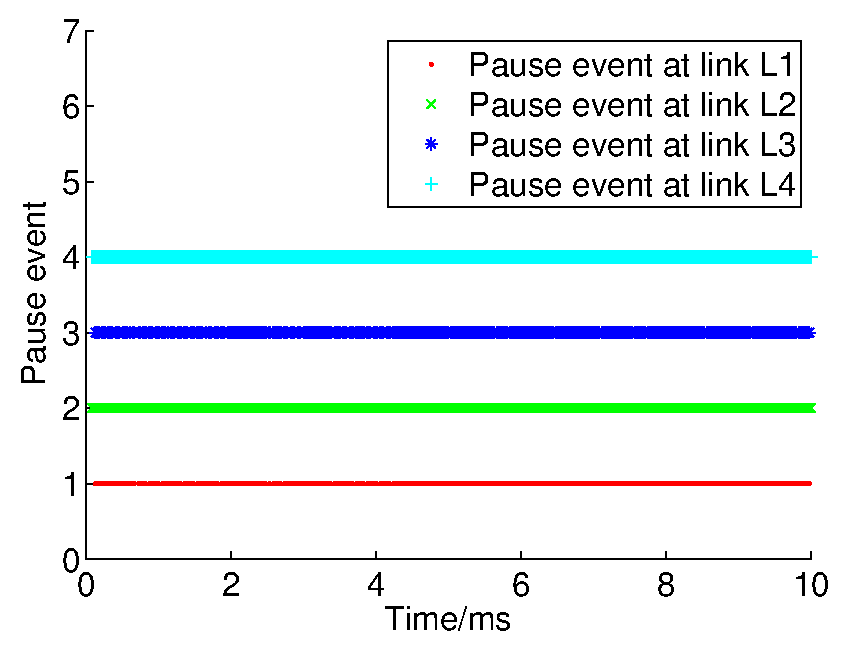
\includegraphics[width=0.3\textwidth] {figs/case3_pause.eps}
}

\caption{\fixme{Different rate limiting determines whether the deadlock may happen.}.}
\label{fig:case3}
\end{figure*}

\subsection{Case 3: Rate Limiting Mitigates Deadlock}

In the last deadlock example (Figure~\ref{fig:case2}), if we additionally rate-limit flow 3, deadlock
may be avoided.  As shown in Figure~\ref{fig:case3}(a), we add a rate limiter to switch C's
outgoing port TX2. This rate limiter on switch C pushes back flow 3 by generating PFC PAUSE
at port RX2 towards switch B (and switch B further pushes back the host). 
Note that the PAUSE of flow 3 at L2 can cause Head-of-Line (HoL) blocking for flow 1 packets on
the same link. if this HoL blocking is serious enough, the flow 1 packets can build up a queue 
at at switch B and the PFC may cascade further .As a result, we 
observe frequent PFC PAUSE on all L1, L2, L3 and L4, as shown in Figure~\ref{fig:case3}(b).


We test different rate limiting values, and find that when the rate limit is below \fixme{X},
there is no deadlock even though all links have frequent PAUSE. \fixme{todo}

\if 0
\textbf{Case 3:} In this case, we will show that even if all the four links are paused simultaneously, 
it is not guaranteed that a deadlock will be created. As shown in Figure~\ref{fig:case3}(a), in addition 
to case 1, we add another two flows (flow 3 and flow 4). Flow 3 starts at a host attached to A, passes 
through A and B, and ends at a host attached to B. Flow 4 is a symmetric flow of flow 3 that runs over 
C and D. All the four flows are UDP flows with infinite traffic demand. Two rate limiters are added at 
TX3 queues of B and D to ensure that rates of flow 3 and flow 4 will not exceed $1/4$ of the link 
capacity. Buffer dependency graph of case 3 is drawn in Figure~\ref{fig:case3}(b). Compared with case 1, 
two additional buffer dependencies from TX1 queues to TX3 queues are added.

Pause events at four links L1, L2, L3 and L4 are plotted In Figure~\ref{fig:case3}(c).  As we can see 
from the figure, all the four links are paused continuously. However, we find that once we stop the 
flows, all the links get resumed and buffer occupancy of four switches soon becomes zero. This 
indicates that deadlock cannot be created in case 3.

To find out why there is no deadlock in case 3, we draw the instant buffer occupancy of 3 flows at 
switches A and B in Figure~\ref{fig:case3}(d), Figure~\ref{fig:case3}(e) and Figure~\ref{fig:case3}(f). 
Here we omit the buffer occupancy condition of switches C and D as the topology and the flows are symmetric.

As shown in Figure~\ref{fig:case3}(d), at TX1 of A, the buffer occupancy of flow 2 exceeds the PFC 
threshold, so link L4 will get paused. To understand why link L1 is also paused, we need to consider 
the buffer occupancy of flow 1 and flow 3 at switch B. The reason is that packets received by RX1 of 
B are possible to be queued at both TX1 and TX3 (note that there is a rate limiter on TX3). As long 
as the sum of the buffer occupancies of both TX queues exceeds the PFC threshold, link L1 will get paused. 
As we can see in Figure~\ref{fig:case3}(e) and Figure~\ref{fig:case3}(f), although individually buffer 
occupancy of either TX1 or TX3 is less than the PFC threshold, their sum is larger than the PFC 
threshold. Hence link L1 is paused.

As both TX1 and TX3 contribute to the pause on link L1, to create a deadlock, we need to ensure that 
packets buffered at both TX queues cannot get resumed. However, packets buffered at TX3 can always get 
transmitted within a finite time as it is not involved in any cyclic buffer dependency. This explains 
why when we stop the flows, all the four links can be resumed from the pauses. 
\fi

%\textbf{Observation 3:} even if all the links in a cycle are paused simultaneously, it is not 
%sufficient to create a permanent deadlock.

\para{Summary:} From all the examples in this section, we summarize that cyclic buffer dependency is
 a loose condition for deadlock. The traffic demand matrix, TTL and flow rates all affect the deadlock
 occurrence. While we cannot obtain the tightest condition ({\em i.e., necessary and sufficient condition}), 
we know that a tighter condition should include those factors, and that these factors can be utilized
for deadlock mitigation. In Section~\ref{sec:mitigation}, we discuss potential deadlock mitigations in 
addition to avoiding cyclic buffer dependency.

%\subsection{Deadlock problem in RDMA DCNs}\label{subsec:deadlock_problem}
%
%Once a loop occurs in a network, packets of some flows will be caught in the loop and traverse the same links multiple times until they are dropped due to Time-to-Live (TTL) expiration. Apart from causing packet drops, loops will also waste some link bandwidth as well as increase the end-to-end delay for the flows traversing some link(s) in the loop (but not caught by the loop).
%
%\begin{figure}[t]
%\centering
%\includegraphics[width=0.45\textwidth,center]{figs/deadlock_example.pdf}
%\caption[Optional caption for list of figures]{An example of loop induced deadlock: there is a loop between switch A and switch B. Both TX queues (egress queues) are paused by PFC as no buffer are available at both switches to accommodate more packets.}
%\label{fig:loop_deadlock}
%\end{figure}
%
%In a lossy network, the impact of a loop is not fatal and can be completely eliminated as long as the loop is removed from the network. In contrast, in a lossless network, if packets enter a loop faster than they get dropped in the loop due to TTL expiration, packets will occupy the buffer of all the switches in the loop, and then a deadlock is created. When a deadlock occurs, each switch in the loop is paused by its downstream switch, and at the same time pauses its upstream switch due to the lack of available buffer to accept more packets. Once such a circular buffer dependency is created, the deadlock condition will hold persistently even after the loop is eliminated.
%
% Under deadlock condition, no packets can move along the links in the loop, and more and more devices outside the loop will be paused due to the cascade effect of PFC. If a deadlock is created in the core of the network, it is very likely to bring the whole data center into a deadlock state.
%
%A simple deadlock example is shown in Figure~\ref{fig:loop_deadlock}. In this example, there is a routing loop between switch A and switch B. Packets enter this loop at a sufficient large rate and soon occupy all the available buffer of both switches. Then Both TX queues (egress queues) will be paused by PFC PAUSE frames and a deadlock is created. As we can see, this deadlock cannot be resolved by eliminating the routing loop as packets are already queued in the TX queues and can never reach the next-hop switch to escape from the loop.
%
%\subsection{Sufficient condition for deadlock creation}\label{subsec:deadlock_condition}
%
%In this part, we analyze the sufficient condition to create a deadlock when there is a loop in the network.
%
%At first, we consider the maximum packet drain rate in a loop regarding TTL expiration. Let $n$ the number of switches in a loop, $B$ be the link bandwidth and $k_{TTL}$ be the TTL value of packets before they enter the loop. Each time a packet traverses one switch, its TTL value will be reduced by 1.
%
%The maximum packet drain rate is achieved when no switch is paused by PFC PAUSE frame and each switch is sending packets to its next-hop in the loop at the rate of $B$. So the maximum packet drain rate $r^{max}_d$ is equal to $nB/k_{TTL}$. here $nB$ can be viewed as the maximum packet ``flowing" rate in the loop, while $1/k_{TTL}$ captures the information that a packet will be dropped after it has traversed $k_{TTL}$ hops of switches in the loop.
%
%Let $r_{in}$ be the injection rate of packets into the loop. One sufficient condition to create a deadlock in a lossless network is that: there is a loop
%in the network, and condition $r_{in} > r^{max}_d$ holds for a sufficient long period until a circular buffer dependency is created in the loop.
%
%\begin{figure}[t]
%\centering
%\includegraphics[width=0.5\textwidth,center]{figs/r_and_rdrain.pdf}
%\caption[Optional caption for list of figures]{Measurement of the minimum injection rate to create a deadlock. Both switches in the loop are Arista 7050QX32.}
%\label{fig:mrate_measurement}
%\end{figure}
%
%To verify our analysis above, we manually configure a loop between two 40Gbps switches, and measure the minimum packet injection rate that can create a deadlock. The result is shown in Figure~\ref{fig:mrate_measurement}. As we can see, the measured minimum packet injection rate is just slightly larger than the maximum packet drain rate which is computed according to $nB/k_{TTL}$. This observation holds when TTL is set to different values.
%
%Another observation from the figure is that, setting smaller TTL can help to prevent deadlock but its benefit is limited. As shown in the figure, when TTL is set to 16 which is already a very small value, the minimum injection rate is only about 6Gbps.
%
%\subsection{Analysis of the time to create a deadlock}\label{subsec:deadlock_condition}
%
%In this part, we analyze and measure the time to create a deadlock when the sufficient condition for deadlock creation is already met. Deadlock creation time is related to three factors: \textbf{packet injection rate $r_{in}$}, \textbf{packet drain rate $r_{d}$} and \textbf{PFC threshold $t_{PFC}$}.
%
%$t_{PFC}$ determines the minimum bytes of packets needed to be ``trapped" in the loop to create a deadlock, while $r_{in} - r_{d}$ can be viewed as the packet increase rate.
%
%%Packet injection rate is determined by the instant traffic demand of applications running in the data center. A larger injection rate requires less time to create a deadlock.
%%
%%As discussed above, the maximum packet drain rate will be a fixed value once $n$, $B$ and $k_{TTL}$ is determined. We find that packet drain rate will decrease significantly after packets are queued in the loop because it will take a packet much longer time to get dropped in the loop when there is queuing delay.
%
%Most modern commodity switches use a dynamic $\alpha$ algorithm to determine the value of PFC threshold: Let $\alpha$ be a parameter with the range from 0 to 1, $m$ be the total switch buffer size and $m^\prime$ be the amount of buffer currently occupied. For a given $\alpha$, the value of $t_{PFC}$ is dynamically computed according to the following equation $ t_{PFC} = \alpha(m - m^\prime)$. During runtime, once the queue length of an ingress queue exceeds the instant $t_{PFC}$, a PAUSE frame will be sent to its upstream device. Note that a PAUSE frame will take some time to arrive an upstream device and take effect. To avoid packet loss due to this delay, some buffer headroom must be reserved for each ingress queue, and hence the value of $m$ in the equation is usually slightly smaller than the total switch buffer size.
%
%%
%
%
% %Most modern commodity switches share memory buffer among all ports. In order to better utilize the available shared buffer in a timely fashion, instead of setting a fixed PFC threshold,
%%A PAUSE frame will take some time to arrive an upstream device and take effect. To avoid packet loss due to this propagation delay, we must reserve enough
%%buffer headroom for each ingress queue to accommodate packets a switch may receive before a PAUSE frame finally takes effect. Let $\Delta m$ be the total amount of reserved buffer headroom. The $m$ in the above equation should be modified to be $m - \Delta m$.
%%Switches and NICs will track the value of $m^\prime$ and update the value of $t_{PFC}$ during runtime.
%
%%A smaller $\alpha$ value can lead to a shorter creation time of deadlock.  This is because a smaller $\alpha$ value means a smaller PFC threshold, while a smaller PFC threshold requires less packets to trigger a switch queue to send PAUSE frames to stop its upstream neighbors.
%
%In the next, we measure the time to create a deadlock when setting different $\alpha$ and TTL values.
%
%
%\begin{figure}[t]
%\centering
%\includegraphics[width=0.5\textwidth,center]{figs/r_dltime.pdf}
%\caption[Optional caption for list of figures]{Measurement of the time to create a deadlock under different settings (deadlock will not occur when the injection rate is less than 1.3Gbps).}
%\label{fig:dltime_measurement}
%\end{figure}
%
%\parab{Measurement of the time to create a deadlock:} We manually configure a loop between two Arista 7050QX32 switches which have 32 full duplex 40Gbps ports and 12MB shared buffer. In Figure~\ref{fig:dltime_measurement}, we set $\alpha$ and $TTL$ to different values and measure the time to create a deadlock under different injection rates.
%
%We can make four observations from the results in Figure~\ref{fig:dltime_measurement}: 1) It takes only a few milliseconds to create a deadlock even when the injection rate is less than 2Gbps. This indicates that it is easy for a deadlock to occur even when only a transilient loop exists in the network. In addition, we cannot rely on any loop detection and recovery solutions to prevent the occurance of deadlocks as they are too slow to resolve the loop within a few milliseconds. 2) As the injection rate increases, the time to create a deadlock decreases accordingly. 3) Given a fixed injection rate, a smaller $\alpha$ value requires less time to create a deadlock. 4) Given a fixed injection rate, a smaller TTL value requires more time to create a deadlock. This is because a smaller TTL value will make the packets get dropped faster in the loop, and thus more packets are needed to be injected into the loop to trigger switch to pause each other.
%
%We repeated this experiment using many other combinations of TTL and $\alpha$ values and different number of switches. We found that all the results comply with what have been shown in Figure~\ref{fig:dltime_measurement}.
%
%The takeaway of this experiment is that: once there is a loop in the network, deadlock is easy to occur and very hard to prevent (a deadlock can be created within a few milliseconds). In addition to a fast loop detection mechanism, we need an effective solution to detect and resolve deadlocks caused by all kinds of loops.

%\parab{Estimation of the time to create a deadlock:}

%\parab{Sufficient condition for deadlock creation:} \todo{(detailed content to be added later.)}
%
%   1. Analysis of the maximum packet drain rate caused by TTL expiration: $r^{max}_d = nB/k_ttl$.
%
%   2. Using testbed experiments to demonstrate that $r > r^{max}_d$ is a sufficient condition for deadlock creation.
%
%\parab{Creation time of deadlock:} \todo{(detailed content to be added later.)}
%
%   1. Analysis of the upper bound and lower-bound of the creation time of deadlock.
%
%   2. a) Using testbed experiments to demonstrate that lower-bound value is already a tight estimation when $r << B$; b) Analysis of the impact of PFC PAUSE frames on $r$ and $r^{max}_d$.
%
%\subsection{Analysis of device bug induced deadlock}\label{subsec:analysis_loop_deadlock}
%\todo{to be added.}

\section{Solution}\label{sec:solution}

In this part, we present our preliminary solution for achieving fast deadlock-free routing reconfiguration.

During the routing reconfiguration process, to avoid routing blackhole~\cite{everflow} and transient routing loop~\cite{dionysus}, each packet should be forwarded either using the rules prior to the reconfiguration, or the rules after the reconfiguration, but never a mixture of the two. This is called \textit{per-packet consistency}. To implement such an abstraction, a two-phase commit mechanism was proposed~\cite{abstractionforupdate}. This mechanism guarantees atomic configuration of a single path. In our solution, we follow the widely adopted two-phase commit mechanism~\cite{abstractionforupdate,zupdate,dionysus}, and assume the routing reconfiguration is performed at the path level instead of the single rule level.


\subsection{Configuration Dependency Graph}\label{subsec:cdg}

\begin{figure}[t]
	\centering
	\includegraphics[width=0.45\textwidth] {figs/CDG}
	\caption{Representing the two deadlock-free reconfiguration schemes in Fig~\ref{fig:treecase}(f) using two configuration dependency graphs.}\label{fig:cdg}
	\vspace{-0.15in}
\end{figure}

\begin{figure}[t]
	\centering
	
	\subfloat[short for lof][Topology and path.] {
		\includegraphics[width=0.22\textwidth] {figs/relationship_or_a}
	}
	\subfloat[short for lof][Deadlock-free scheme and Corresponding CDG.]{
		\includegraphics[width=0.24\textwidth] {figs/relationship_or_b}
	}
	
	
	\caption{An example to show the OR relationship. Node $oi$ is the operation to configure path $pi$.}\label{fig:orrelationship}
	\vspace{-0.2in}
\end{figure}

In this part, we define \textit{configuration dependency graph} (CDG) to represent any possible routing reconfiguration schemes at the path level. CDG is a directed graph $G_c(V_c,E_c)$, where each node in $V_c$ represents a configuration operation, and each edge in $E_c$ represents an operation dependency. 

In Fig.~\ref{fig:cdg},  we use two CDGs to represent the two deadlock-free reconfiguration schemes in Fig~\ref{fig:treecase}(f). In the first reconfiguration scheme, it requires paths $p1$ and $p2$ to be removed before paths $p3$ and $p4$ are added, hence we use four edges $o1\rightarrow o3$, $o1\rightarrow o4$, $o2\rightarrow o3$, $o2 \rightarrow o4$ in CDG 1 to capture the order dependencies among operations. In the second reconfiguration scheme, it only requires paths $p2$ to be removed before path $p3$ is added. So only one edge $ o2 \rightarrow o3$ is needed in CDG 2.
 


In order to represent any possible routing reconfiguration schemes, our CDG should be able to describe both the ``OR" and ``AND" relationship that could be used in a reconfiguration scheme, as we are going to explained in the next.

\textbf{OR relationship}: It refers to the dependency relationship that a path can be added after any path in a path set is removed. In Fig.~\ref{fig:orrelationship}, we use an example to illustrate this OR relationship. Fig.~\ref{fig:orrelationship}(a) includes a 4-switch network and four paths $p1$, $p2$, $p3$ and $p4$, where $\{p1, p2, p3\}\subseteq 
R_{old}$ and $\{p4\}\subseteq R_{new}$. In Fig.~\ref{fig:orrelationship}(b), a feasible deadlock-free reconfiguration scheme is presented. In order to avoid cyclic buffer dependency, the scheme requires that at least one path in $\{p1, p2, p3\}$ should be removed before path $p4$ is added. This is the "OR" relationship that could be used in a reconfiguration scheme.

To capture the ``OR" relationship in the CDG, we can duplicate the operation that ``partially" depends on other operations into several mirror operations. As shown in the CDG of Fig~\ref{fig:orrelationship}(b), operation o4 is duplicated into three mirror operations o4, o4' and o4''. Operations $o1$, $o2$ and $o3$ are pointed to different mirror operations of $o4$. During the reconfiguration process, as long as one operation in $\{o1, o2, o3\}$ finishes, the operation to add path $p4$ can start immediately as one of the three mirror operations is released.


\begin{figure}[t]
	\centering
	
	\subfloat[short for lof][Topology and path.] {
		\includegraphics[width=0.24\textwidth] {figs/relationship_and_a}
	}
	\subfloat[short for lof][Deadlock-free scheme and Corresponding CDG.]{
		\includegraphics[width=0.24\textwidth] {figs/relationship_and_b}
	}
	
	
	\caption{An example to show the AND relationship. Node $oi$ is the operation to configure path $pi$. }\label{fig:andrelationship}
	\vspace{-0.2in}
\end{figure}

\textbf{AND relationship}: It refers to the dependency relationship that a path can be added after all the paths in a path set are removed. In Fig~\ref{fig:andrelationship}, we use an example to illustrate this AND relationship. As shown in Fig.~\ref{fig:andrelationship}(a), five paths $p1$, $p2$, $p3$, $p4$ and $p5$ traverses a 4-switch network. Both path $p4$ and $p5$ go through S4, S1 and S2 consecutively, but ends at different hosts (not drawn in the figure). In this example, we have $\{p4, p5\}\subseteq R_{old}$ and $\{p2\}\subseteq R_{new}$. Paths $p1$, $p3$ are not involved in the routing reconfiguration.  In Fig.~\ref{fig:andrelationship}(b), a feasible deadlock-free reconfiguration scheme is presented. In order to avoid cyclic buffer dependency, the scheme requires that both of paths $p4$ and $p5$ to be removed before path $p2$ is added. This is the "AND" relationship that could be used in a reconfiguration scheme.

To capture the ``AND" relationship in a CDG, we can let multiple operations point to a single operation, as shown  in the CDG of Fig~\ref{fig:andrelationship}(b). During the reconfiguration process, operation $o2$ will start only after both operations $o4$ and $o5$ finish.

\subsection{Construction of Deadlock-free Configuration Dependency Graph}\label{subsec:dfcdg}

In this part, we present our solution for constructing deadlock-free CDGs. We will also show that if the time to configure a single path can be known in advance or can be accurately estimated, the fastest deadlock-free CDG can be constructed in polynomial time.

Our solution is designed based on the following important observation: \textit{For any cycle in the network, as long as an old buffer dependency edge is permanently removed from the cycle before a different new buffer dependency edge is added to the cycle, there will be no cyclic buffer dependency in the cycle during the routing reconfiguration process.}

This observation can help us to ensure deadlock-free without removing all the paths in $R_{old}$ at first. Before we introduce our solution, we define a few notations used in our solution.

Buffer dependency edges are among ingress queues. As a network link is exactly corresponding to an ingress queue, we use $d_{lx,ly}$ to denote the buffer dependency edge from the ingress queue connected with link $lx$ to the ingress queue connected with link $ly$. We denote a buffer dependency $d_{lx,ly}$ as $d^{o}_{lx,ly}$, if it is created by a path in $R_{old}$. And as $d^{n}_{lx,ly}$ if it is created by a path in $R_{new}$.

We use $D_{o}$ to denote the set of all buffer dependency edges related to the paths in $R_{old}$, and $D_{n}$ to denote the set of all buffer dependency edges related to the paths in $R_{new}$. $O(d^{o}_{lx,ly})$ is the set of operations that can remove the buffer dependency edge $d^{o}_{lx,ly}$ from the network, and $O(d^{n}_{la,lb})$ is the set of operations that can add the buffer dependency edge $d^{n}_{la,lb}$ to the network.



Our solution consists of 3 steps as follows.

\textbf{Step-1: Building $D_{o}$ and $D_{n}$.} We enumerate all the paths in $R_{old}$ and $R_{new}$ to build $D_{o}$ and $D_{n}$. If a buffer dependency edge included in $D_{o}$ is also included in $D_{n}$, we delete it from $D_{o}$ as this edge cannot be permanently removed.

\textbf{Step-2: Constructing a raw deadlock-free CDG.}  For every pair of edges ($d^{o}_{lx,ly}$,  $d^{n}_{la,lb}$), to ensure $d^{o}_{lx,ly}$ is removed from the cycle before  $d^{n}_{la,lb}$ is added to the cycle in the raw CDG, we perform two actions. 

First,  for any operation $oi$ in $O(d^{o}_{lx,ly})$, we create a mirror operation denoted as $oi'$ in the raw CDG. Do the same for any operation $oj$ in $O(d^{n}_{la,lb})$ (denoted as $oj'$).  Second, we add a dependency edge from $oi'$ to $oj'$ for every such pair of operations.

\textbf{Step-3: Deriving deadlock-free CDG(s) from the raw deadlock-free CDG.}  For each connected subgraph in the raw CDG we construct in step-2,  its operation dependency edges ensure that one old buffer dependency edge is permanently removed from a cycle before a new buffer dependency edge is added to the same cycle. This means that each subgraph stand alone can ensure deadlock-free for a certain cycle.  

Assuming the network contains $n$ cycles, a deadlock-free CDG can be created by picking $n$ subgraphs from the raw CDG,  with each subgraph corresponding for a cycle in the network. Different combinations is corresponding to different deadlock-free CDGs.

\textbf{Calculation of fastest deadlock-free CDG}: If the time of any single configuration operation is already known, then we can easily calculate the total configuration time of any subgraph in the raw CDG. In this case, By choosing a subgraph with minimum configuration time for each cycle, we can produce a fastest deadlock-free CDG in polynomial time.

\begin{figure}[t]
	\centering
	
	\subfloat[short for lof][Topology and paths.] {
		\includegraphics[width=0.26\textwidth] {figs/solution_example_a} 
	}
	\subfloat[short for lof][Raw CDG and Fastest CDG.] {
		\includegraphics[width=0.22\textwidth] {figs/solution_example_b}
	}
	
	\caption{An example to illustrate the solution. In this example, we simply assume the time cost to configure a path is equal to the number of switches this path traverses.}\label{fig:solution_example}
	\vspace{-0.2in}
\end{figure}

In Fig.~\ref{fig:solution_example}, we have an example to show how our solution works. As shown in Fig.~\ref{fig:solution_example}(a), there are four paths traversing a 4-node network. We have $\{p1, p3\}\subseteq R_{old}$ and $\{p2, p4\}\subseteq R_{new}$. It is easy to calculate $D_{o}=\{d^{o}_{l1,l2},  d^{o}_{l3,l4}\}$, and $D_{n}=\{d^{n}_{l2,l3},  d^{n}_{l3,l4},  d^{n}_{l4,l1}\}$.  According to the algorithm in step-1, $d^{o}_{l3,l4}$ will be deleted from $D_{o}$ as we have $d^{n}_{l3,l4}$ in $D_{n}$.

For all the remaining buffer dependency edges, their corresponding operations are as follows: $O(d^{o}_{l1,l2}) = \{o1\}$, $O(d^{n}_{l2,l3}) = \{o2\}$, $O(d^{n}_{l3,l4}) = \{o2\}$ and $O(d^{n}_{l4,l1}) = \{o4\}$. Then according to step-2, for every pair of edges ($d^{o}_{lx,ly}$,  $d^{n}_{la,lb}$), we create some mirror operations as well as the corresponding dependency edges in the raw CDG. The raw CDG can be found in Fig~\ref{fig:solution_example}(b) (Note that one redundant subgraph $o1'' \rightarrow o2'$ is not drawn).  

As we can find, every connected subgraph in the raw CDG exactly removes one old buffer dependency edge from the cycle before adding a new buffer dependency edge to the  cycle. Hence we can derive two deadlock-free CDGs from the raw CDG: CDG 1 only includes the dependency $o1\rightarrow o2$, while CDG 2 only includes the dependency $o1'\rightarrow o4$.

As shown in Fig.~\ref{fig:solution_example}, if we know the time of any single operation, the total configuration time of any subgraph in the raw CDG can be easily calculated. For example, operations in subgraph $o1 \rightarrow o2$ needs 7 time units to finish, while operations in subgraph $o1' \rightarrow o4$ only needs 6 time units to finish.  Then we can produce a fastest deadlock-free CDG with 6 configuration time, as shown in Fig.~\ref{fig:solution_example}(b).


%\subsection{Fast Deadlock-free Reconfiguration For a Single Cycle}\label{subsec:dfrforsc}
%
%In this part, we present our solution for constructing a deadlock-free CDG $G_c(V_c,E_c)$ for a single topology cycle $C$ in $G(V,E)$. 
%
%The naive approach to find an optimal deadlock-free CDG is to enumerate all the possible CDGs, and choose a deadlock-free CDG with minimum configuration time. However, it would be computationally impossible as there are combinatorial such CDGs. 
%
%Our solution is designed based on the observation that \textit{For a single topology cycle with cyclic buffer dependency, as long as we guarantee that one old buffer dependency edge is removed from the cycle before one different new buffer dependency edge is added to the cycle, the reconfiguration process will be deadlock-free.} 
%
%In the next, we describe how our solution works. For each pair of adjacent links $lx$ and $ly$ in cycle $C$, let $P_s^{lx,ly}$ be the set of paths in $P_s$ contributed to the buffer dependency edge $d_{lx,ly}^{P_s}$, and $P_t^{lx,ly}$ be the set of paths in $P_t$ contributed to the buffer dependency edge $d_{lx,ly}^{P_t}$. Removing all paths in $P_s^{lx,ly}$ will delete buffer dependency edge $d_{lx,ly}^{P_s}$ from the network, while adding paths in $P_t^{lx,ly}$ will create buffer dependency edge $d_{lx,ly}^{P_t}$.
%
%
%For any non-empty set $P_t^{lx,ly}$, as $P_t$ is deadlock-free, there exists at least one 
%
%Given two non-empty sets $P_s^{lx,ly}$ and $P_t^{lm,ln}$ that satisfy $(lx, ly) \neq (lm, ln)$, to guarantee one old buffer dependency edge is removed before one different new buffer dependency edge is added, we can let all the paths in $P_s^{lx,ly}$ be removed from the network before adding any path in $P_t^{lm,ln}$. In other word, we can construct a deadlock-free CDG by adding a configuration dependency edge from any path in $P_s^{lx,ly}$ to any path in $P_t^{lm,ln}$.
%
%In the next, we present our solution for searching deadlock-free CDGs with minimum time cost.  Assuming that we know the time cost to remove or add a single path. Then we can calculate the time cost of path configurations for any $P_s^{lx,ly}$ and any $P_t^{lm,ln}$. To find the optimal CDG(s), our solution will calculate the time cost of path configurations for any legal pair ($P_s^{lx,ly}$, $P_t^{lm,ln}$), and then choose the one with minimum time cost. 
%
%Let $k$ be the number of links in $C$, and $n$ be the number of paths contributed to the buffer dependency in $C$. The time complexity of the above calculation is within $O(nk + k^2)$. Hence our solution is scalable.
%

%In Fig.~\ref{fig:solution_example1}, we use a simple example to illustrate how our solution works. In this example, $P_s=\{p1, p3\}$ and $P_t=\{p2, p4\}$. As we can see in Fig.~\ref{fig:solution_example1}(a), paths in $P_s \cup P_t$ introduce a cyclic buffer dependency to the network. It is easy to know $P_s^{l1,l2} = \{p1\}$, $P_s^{l3,l4} = \{p3\}$, $P_t^{l2,l3} = \{p2\}$, $P_t^{l3,l4} = \{p2\}$ and $P_t^{l4,l1} = \{p4\}$.
%
%Let $t_{add}(p)$ and $t_{rmv}(p)$ be the time cost to add and remove a path p, respectively. In this example, we assume  the time cost to configuring a path is equal to the number of switches this path traverses in the cycle. So we have $t_{rmv}(p1)=3$, $t_{add}(p2)=4$, $t_{rmv}(p3)=3$ and $t_{add}(p4)=4$.
%
%Our solution will calculate the time cost for all the path sets contributed to some buffer dependency edge. The results are as follows $t(P_s^{l1,l2}) = 3$, $t(P_s^{l3,l4}) = 3$, $t(P_t^{l2,l3}) = 4$, $t(P_t^{l3,l4}) = 4$, $t(P_t^{l4,l1}) = 3$.
%
%Our solution will then calculate the time cost of path configurations for any pair ($P_s^{lx,ly}$, $P_t^{lm,ln}$), and then choose one optimal pair with minimum time cost. In this example, both ($P_s^{l1,l2}$, $P_t^{l4,l1}$) and ($P_s^{l3,l4}$, $P_t^{l4,l1}$) have minimum time cost, so two optimal CDGs can be constructed, as shown in Fig.~\ref{fig:solution_example1}(b). 
%

%The intuition behind our solution is that \textit{For each possible cycle in the buffer dependency graph, as long as we ensure that one old dependency link is removed before one new dependency link is added, the reconfiguration process is deadlock-free.} 
%
%The idea of our heuristic solution is as follows: First, for each cycle in the buffer dependency graph, we enumerate all the sets of update actions that can exactly add or remove one dependency link from the graph. Then we pick up two minimum action sets A and B, where A can remove one dependency link for a given cycle while B can add an dependency link for the same cycle. The deadlock-free reconfiguration scheme our solution produces will ensure that A is finished before B starts to be configured.

%shows an example of CDG. In the graph, each node represents a configuration operation. For example, node $o1$ represents the operation to remove path $p1$, while node $o3$ represents the operation to add path $p3$. Each directed edge in the graph represents an order constraint on the operations. For example,  $o1$ must be finished before we start the operation $o4$.

%Let $P_c$ be the set of configuration paths in $G_c$. In Fig.~\ref{fig:cdgraph}, there are three legal configuration paths: 1) o1-o3; 2) o1-o4; 3) o2-o3. 
%
%We use $ts(G_c)$ to denote a topological sorting of $G_c$. $ts(G_c)$ represents a possible order of configuration operations in terms of the finish time.  $TS(G_c)$ is the set of all possible topological sortings in $G_c$. In Fig.~\ref{fig:cdgraph}, there are five possible topological sortings: (o1, o2, o3, o4), (o1, o2, o4, o3), (o1, o4, o2, o3), (o2, o1, o4, o3) and (o2, o1, o3, o4). $P^{(i)}(ts)$ is  the set of active routing paths after first i-th operations in $ts(G_c)$ is finished.

%\subsection{Problem Formulation}\label{subsec:formulation}
%
%\begin{table}
%	\begin{tabularx}{0.48\textwidth}{ |c||X| } 
%		\hline
%		$G(V,E)$ & The DCN, where $V$ is the set of all nodes and $E$ is the set of all links. \\ 
%		\hline
%		$C$ & $C \subset G(V,E)$ is a cycle in $G(V,E)$. \\ 
%		\hline
%		$P_s$ & The set of paths in the old configuration. \\
%		\hline
%		$P_t$ & The set of paths in the new configuration. \\
%		\hline
%		%	$R_s$ & The set of rules corresponding to $P_s$. \\
%		%	\hline
%		%	$R_t$ & The set of rules corresponding to $P_t$. \\
%		%	\hline
%		%	$V_p$ & The set of nodes on path p. \\
%		%	\hline
%		%	$E_p$ & The set of links on path p. \\
%		%	\hline
%		$R_p$ & The set of rules corresponding to path p. \\
%		\hline
%		
%		$G_c(V_c,E_c)$ & A configuration dependency graph, where $V_c$ is a set of configuration operations, and $E_c$ is a set of order dependencies.\\
%		\hline
%		$P_c$ & The set of configuration paths in $G_c$.\\
%		\hline
%		%	$t_o$ & The time to finish an operation $ o \in V_c$.\\
%		%	\hline
%		$t(P, G_c)$& The time to configure all paths in $P$ obeying the dependencies in $G_c$.\\
%		\hline
%		$ts(G_c)$ & A topological sorting of $G_c$, which is a list of configuration operations. \\ 
%		\hline
%		$TS(G_c)$ & The set of all possible $ts(G_c)$. \\
%		\hline
%		$P^{(i)}(ts)$& The set of active paths after finishing first i-th operations in $ts(G_c)$.\\
%		\hline
%		%	$P_s^{(i)}(ts)$& The set of remaining paths in $P_s$ after finishing first i-th operations in $ts(G_c)$.\\
%		%	\hline
%		%	$P_t^{(i)}(ts)$& The set of activated paths in $P_t$ after finishing first i-th operations in $ts(G_c)$.\\
%		%	\hline
%		$d_{lx,ly}^P$ & The buffer dependency edge from link l1 to link l2 introduced by the paths in $P$.\\
%		\hline
%		$P^d_{lx,ly}$ & The set of all paths in $P$ contributed to  $d_{lx,ly}^P$.\\
%		\hline
%	\end{tabularx}
%	\caption{The key notations used in the problem formulation.}\label{table:formulation}
%\end{table}
%
%
%
%
%In Table~\ref{table:formulation}, we list the key notations used in our problem formulation. $G(V,E)$ is the DCN topology. $C$ is a cycle in $G(V,E)$.  $P_s$ is the set of old routing paths, while $P_t$ is the set of new routing paths. Here we assume $P_s \cap P_t = \emptyset$, which can always be achieved by removing all the paths in $P_s \cap P_t$ in advance.

%$R_s$ and $R_t$ are the set of rules corresponding to the paths in $P_s$ and $P_t$, respectively.  $R_p$ is the set of rules for path p. 

% $t_p$ is the time to configure path $p$ (if $p$ is an old path, the operation is to add path $p$. Otherwise, it is to remove path $p$.

%We define $t(P, G_c)$ as the time to configure all routing paths in $P$ with respect to the dependency contrsints in the CDG $G_c$. The value of $t(P, G_c)$ is determined by the bottleneck configuraton path in $G_c$ which requires longest time to finish.
%
%We use $d_{lx,ly}^P$ to denote the buffer dependency from link $lx$ to link $ly$ introduced by the paths in $P$. Note that each link in a DCN is exactly corresponding to an ingress queue. For simplicity, we use a pair of links to denote the buffer dependency among a pair of ingress queues.  We define
%
%\begin{equation} \label{eq:1}
%d_{lx,ly}^P = \left \{
%\begin{aligned}
%&1, && \text{links } lx \text{ and } ly\text{ are adjacent, and } \exists p \in P\\
%&    &&  \text{ that goes over } lx \text{ and } ly\text{ in sequence.}\\ 
%&0, && \text{otherwise.}
%\end{aligned} \right.
%\end{equation} 
%
%
%%We use $P^d_{l1,l2}$ to denote the set of all paths in $P$ contributed to the buffer dependency $d_{l1,l2}^P$.
%
%Given a DCN topology $G(V,E)$, an old path set $P_s$, a new path set $P_t$ and a CDG $G_c(V_c,E_c)$,  we say $G_c(V_c,E_c)$ is a deadlock-free CDG for the  reconfiguration from $P_s$ to $P_t$ when the following condition is met: for any legal topological sorting $ts(G_c)$, at any reconfiguration state ${P^{(i)}(ts)}$, there is no cyclic buffer dependency for any cycle C in $G(V,E)$. This condition can be formally described as
%
%\begin{equation}  \label{eq:2}
%\begin{split}
%\forall ts \in TS(G_c), \forall P^{(i)}(ts), \forall C \subset G(V,E), \\
%\displaystyle{\prod\limits_{\forall lx, ly \in V(C)} d_{lx,ly}^{P^{(i)}(ts)} =0}
%\end{split}
%\end{equation} 
%
%For an input ($G(V,E)$, $P_s$, $P_t$), The goal of our solution is to find a deadlock-free CDG $G_c(V_c,E_c)$ with minimal reconfiguration time $t(P, G_c)$.

\secspacelarge
\section{Related Work}
\secspace

\para{RDMA in datacenters.} RDMA has been used for improving distributed application performance,
like in-memory key value store~\cite{mitchell13atc, farm, kalia14sigcomm}, 
Hadoop RPC~\cite{hadooprdma} and HBase~\cite{hbaserdma}.
It has been recently deployed inside modern datacenters~\cite{timely,dcqcn,rdmascale}, based on
RoCE (RDMA over Converged Ethernet), which relies on PFC creating a lossless Ethernet.
Recent works~\cite{timely,dcqcn} discuss the transport congestion control protocols. However,
how to prevent PFC deadlock from happening in the lossless Ethernet has been pointed out 
but not well addressed. In this paper, we aim to get deeper understanding on deadlock 
and possible mitigations.

\para{Deadlock-free routing.} To avoid deadlock in lossless networks, previous
work~\cite{tcpbolt,karol2003prevention,lash,sancho2004,wu2003fault} has focused
on deadlock-free routing: i.e. deadlock freedom regardless of traffic pattern
etc. It has also been proven that that eliminating cyclic buffer dependency is a
necessary and sufficient condition for deadlock-free
routing~\cite{deadlockfree}. However, deadlock-free routing is difficult to
implement in practice -- since it is challenging to eliminate cyclic buffer
dependency in face of arbitrary bugs and failures. Our work explores how we may
control the flows, packet formats and switch configurations to avoid deadlock
even if routing is not deadlock-free.







\secspacelarge
\section{Conclusion}
\secspace

In this paper, we studied the problem of deadlock in datacenter networks.  We
showed that CBD is a {\em necessary} by not {\em
sufficient} condition for deadlock formation. We are unable to fully characterize
the sufficient conditions, but using insights gained from a few examples, we
discussed potential deadlock mitigation mechanisms including TTL-based schemes,
rate limiting and reducing PFC propagation.


%\vspace{0.1in}
%\section*{Acknowledgements}


%\begin{normalsize}
\begin{small}
\bibliographystyle{plain}
\bibliography{reference}
\end{small}
%\end{normalsize}
%\begin{appendices}
\section{PFC headroom calculation}\label{APPHEADROOM}

The PFC headroom needed per port per lossless class can be calculated by considering the time interval needed for a receiver to pause its upstream sender. The time interval is composed of the following 6 periods for the lossless class $p$:

\begin{enumerate}
	
\item\textbf{The time to send a PAUSE frame $t_1$}. 
Once a pause frame is generated, it may be blocked by a packet ahead of it which just starts transmitting. Since Ethernet is non-preemptive, the pause fame has to wait for the completion of the previous packet. Hence in the worst-cast, $t_1 = \frac{ L_{mtu} + L_{pfc}}{B}$, where $L_{mtu}$ is the MTU size, and $L_{pfc}$ is the size of a PFC pause frame, and $B$ is the link rate. 

%The transmission of the PAUSE frame  can pass ahead of any other packet queued in the receiver, but cannot preempt another frame currently being transmitted in the same direction. In the worst case, the receiver generates a PAUSE frame right when the first bit of a maximum-size packet has started engaging the transmission logic. So we have  $t_{snd}=(s_{MTU}+s_{PFC})/r_{l}$, where $s_{MTU}$ is the size of a maximum-size packet, $s_{PFC}$ is the size of PFC PAUSE frame and $r_{l}$ is the line rate of network link.

\item\textbf{The PAUSE frame propagation time $t2$}. This value is decided by the cable length between the sender and receiver. 

\item\textbf{The PAUSE frame receiving time at the sender $t3$}. $t_3=\frac{L_{pfc}}{B}$.

\item\textbf{The PFC response time $t_4$}. This is the amount of time needed for the sender to respond after the pause frame is received. 

\item\textbf{The time for the sender to stop transmitting $t_5$)}. Again, because Ethernet is non-preemptive, when the sender decides to stop transmitting, it needs to finish the packet already gets started. In the worst-case, the packet size can be $L^{p}_{mtu}$, which is the maximum packet size for that lossless class $p$. Hence $t_5 = \frac{L^{p}_{mtu}}{B}$. 

\item\textbf{The time for the pipe to be drained $t_6$}. We know $t_6 = t_2$. 

\end{enumerate}

At a first glance, the headroom size should be $B\times\sum t_i$. 

 To correctly calculate the PFC headroom, we need to further consider the fact that most modern switches divide the switch buffer into cells of fixed size. A buffer cell can only accommodate bytes of a single packet. For example, A 64-byte packet will consume one cell of 100 bytes, and 36 bytes of this cell will remain unused.

 We use $s_{cell}$ to denote the size of buffer cell, and $s_{min}$ to denote the minimum size of a packet. In the worst case, the sender sends packets of minimum size in periods 1,2,3,4 and 6, and packets of maximum size in period 5. Hence
 PFC headroom for a single priority per port is (denoted as $b_{hr}$):


 \begin{eqnarray} \label{eqn:pfcheadroom}
 b_{hr}  & = &  s_{cell}\lceil\frac{(s_{MTU}+2s_{PFC}+2r_{l}t_{wire}+r_{l}t_{pro})}{s_{min}}\rceil \nonumber   \\
 & & +  s_{cell}\lceil\frac{s_{MTU}}{s_{min}}\rceil
 \end{eqnarray}

For typical TCP/IP based RDMA DCNs, we have $s_{MTU}$ = 1500bytes, $s_{min}$ = 64bytes, $s_{PFC}$ = 64bytes, $t_{wire} \leq$ 1.5us and $t_{pro}\le $ 4us. For Broadcom chipset, we have $s_{cell}$ = 208bytes. According to the above equation, for commodity switches like Arista 7050QX32 which has 32 full duplex 40Gbps ports and 12MB buffer, it requires about 3.8MB buffer to support a single lossless priority. Hence only 2 lossless priorities can be supported.
\end{appendices}

\end{document}
